\documentclass{article}

\usepackage{microtype}
\usepackage{graphicx}
\usepackage{booktabs}
\usepackage{amsmath}
\usepackage{amssymb}
\usepackage{hyperref}
\usepackage{amsthm}
\usepackage{enumitem}

\newcommand{\theHalgorithm}{\arabic{algorithm}}

\usepackage[accepted]{icml2018}

\icmltitlerunning{TurnOne: The Cost of Convention in Low-Rank Games}

\begin{document}

\twocolumn[
\icmltitle{TurnOne: The Cost of Convention in Low-Rank Games}

\begin{icmlauthorlist}
\icmlauthor{Lucas Brennan-Almaraz}{su}
\end{icmlauthorlist}

\icmlcorrespondingauthor{Lucas Brennan-Almaraz}{leba@stanford.edu}

\icmlaffiliation{su}{Department of Computer Science, Stanford University, Stanford, CA, USA}

\icmlkeywords{game theory, behavioral cloning, empirical game theory, low-rank games, Pokemon}

\vskip 0.3in
]

\printAffiliationsAndNotice{}

\begin{abstract}
Expert Pok\'emon VGC strategies look nothing like Nash equilibria (total variation 0.99), yet expert-vs-expert outcomes match Nash payoffs within 0.02. Random strategies achieve the same result. SVD of the ${\sim}200$-action payoff matrices reveals effective rank~3, with 93\% of strategic variation in the payoff null space. Switching from behavioral cloning to offline RL (Conservative Q-Learning) confirms that game structure, not the learning objective, is the binding constraint: CQL reshapes 60\% of the distribution but gains only 17\% in exploitability. The one exception is terastallization, an irreversible resource where convention accounts for 30\% of total exploitability; yet in full battles, turn-1 terastallization yields only a 1.7pp win-rate edge over deferring ($n{=}45{,}172$), suggesting the large immediate payoff our model sees is largely offset by strategic costs it cannot represent. The question is not whether experts are rational, but whether the game notices.
\end{abstract}

%% ============================================================
\section{Introduction}
%% ============================================================

Expert Pok\'emon VGC strategies are maximally different from Nash equilibria (TV~$= 0.99$) yet produce identical payoffs against each other (gap~$= -0.02$). Experts do not deserve credit for this: random strategies achieve the same result. The game's structure makes convention free.

We study this in the Video Game Championships (VGC) doubles format. Each player builds a team of six Pok\'emon, brings four to battle, and selects two as leads. On turn~1, both players simultaneously choose actions for their two active Pok\'emon. The action space is combinatorial (${\sim}200$--$400$ valid actions per side), the game is zero-sum and simultaneous, and 154,718 recorded expert battles provide a large behavioral dataset. Our goal is to explain \emph{why} conventional play succeeds, a structural question that agent-building alone cannot answer.

We formalize turn-1 play as an offline contextual bandit (context is the
game state, action is one of ${\sim}200$ valid turn-1 combinations, reward
comes from a learned dynamics model) and ask three questions:

\begin{itemize}[nosep,leftmargin=*]
  \item \textbf{Convention $\neq$ strategy.} How far is expert play from
    optimal? Very far: BC is exploitable by 1.41 reward units and
    TV $= 0.99$ from Nash, yet cross-play outcomes match Nash payoffs
    within 0.02 (\S\ref{sec:convention}).
  \item \textbf{Convention is free.} Why doesn't this matter? Payoff
    matrices have effective rank~3 out of ${\sim}122$ actions, so 93\%
    of strategic variation is payoff-irrelevant (\S\ref{sec:free}). The
    exception is terastallization, an irreversible resource that accounts
    for 30\% of exploitability (\S\ref{sec:tera}).
  \item \textbf{Can reward optimization escape?} Switching from imitation
    to offline RL (CQL) reshapes 60\% of the distribution but gains only
    17\% in exploitability; 94\% of the shift lands in the payoff null
    space (\S\ref{sec:cql}).
\end{itemize}

\subsection{Related Work}

\textbf{Minimax in sports.}
Studies of penalty kicks \citep{chiappori2002testing, palacios2003professionals} and tennis serves \citep{walker2001minimax, anderson2024professionals} find near-minimax play in 2--3 choice domains. Our setting has ${\sim}200$ actions and requires a learned payoff model.

\textbf{Price of anarchy and focal points.}
The price of anarchy \citep{koutsoupias1999worst, roughgarden2002bad} measures the cost of equilibrium play relative to social optimum; we measure the cost of \emph{conventional} play relative to equilibrium. \citet{schelling1960strategy} argued that players coordinate on salient defaults (focal points); our finding that expert conventions are payoff-equivalent to Nash quantifies this for a large action space.

\textbf{Poker AI.}
Superhuman poker agents \citep{bowling2015heads, brown2019superhuman} show that human play is exploitable but focus on building agents rather than characterizing the \emph{structure} of human suboptimality.

\textbf{EGTA.}
Our approach follows the EGTA framework \citep{wellman2006methods}, substituting a learned dynamics model for the traditional simulator oracle.

\textbf{Offline RL.}
Conservative Q-Learning \citep{kumar2020conservative} learns policies from fixed datasets by penalizing Q-values on out-of-distribution actions, avoiding the overestimation that plagues na\"ive offline methods in large action spaces. We use CQL not to build a better agent but as a diagnostic: if reward optimization cannot escape convention, the constraint is structural.

\textbf{Pok\'emon AI.}
VGC-Bench \citep{angliss2025vgcbench} evaluates LLM agents; Metamon \citep{grigsby2025metamon} applies offline RL to singles. Both train agents; we measure existing human play. Prior work has studied low-rank games theoretically and documented human deviations from Nash empirically, but not connected the two. No existing study uses payoff matrix rank to explain why suboptimal play produces Nash-equivalent outcomes in games with hundreds of actions.

%% ============================================================
\section{Approach}
\label{sec:approach}
We instantiate the contextual bandit as follows. Each turn-1 decision has a
context $s$ (team composition, leads, field), an action $a$ from
${\sim}200$ valid combinations, and a reward $r(s,a,a')$ from a learned
dynamics model. Each active Pok\'emon picks one of four moves, each targetable at either opponent or its own partner; the player may also terastallize one Pok\'emon. The joint choice across both active slots produces the ${\sim}200$ combinations. We exclude voluntary switches (${\sim}27\%$ of battles) because a switch changes which Pok\'emon is active, producing a different action space entirely. The horizon-1 structure means $Q(s,a) =
\mathbb{E}[r \mid s, a]$ with no bootstrapping, so CQL reduces to
conservative reward regression. We compare three approaches: behavioral
cloning (BC), which imitates expert play and ignores reward; CQL, which
optimizes reward while staying near the data distribution; and Nash
equilibria, computed via LP on the same reward model's payoff matrix.

\subsection{Data}

We use 154,718 rated battles from Pok\'emon Showdown (Gen~9 VGC Regulation~G, 1500+ Elo), yielding 309,436 directed turn-1 examples \citep{brennan2026turnzero}. Each example encodes full team composition (6 Pok\'emon with moves, abilities, items), lead assignments, and field state. Actions are encoded as 16~slots per Pok\'emon (4 moves $\times$ 4 targets) with a 3-way tera flag.

\subsection{Behavioral Cloning}

Our BC model uses a Transformer encoder (4~layers, 4~heads, $d_\text{model} = 128$) operating on 12~Pok\'emon tokens plus 1~field token. Two heads decode independently: a 16-way action head per active Pok\'emon and a 3-way tera head, with $P(a_1, a_2, \text{tera}) = P(a_1) \cdot P(a_2) \cdot P(\text{tera})$. The model achieves 44.8\% top-1 accuracy ($3\times$ uniform) and 79.6\% top-3 accuracy with 1.32M parameters. We validate the independence assumption in Section~\ref{sec:ablations}: mutual information between leads' actions is 0.018~bits.

\subsection{Dynamics Model}

The dynamics model shares the encoder architecture, adds action embeddings fused with the encoder output, and predicts per-Pok\'emon HP changes, KO probabilities, and post-turn field state. This defines the bandit's reward function $r(s,a,a')$. It achieves HP mean absolute error (MAE) of 13.3/100 and KO area under the ROC curve (AUC) of 0.91.

\textbf{Signal-to-noise validation.} All game-theoretic quantities depend on learned dynamics, so we check that signal exceeds model noise. Injecting Gaussian noise at the dynamics model's reward-space error scale (MAE $= 1.19$) yields a noise-floor exploitability of 0.41, giving a signal-to-noise ratio of 3.4:1 against our measured exploitability of 1.41.

\textbf{Why turn-1 reward?} Turn-1 reward is weakly predictive of battle outcome (point-biserial $r = 0.21$, $n = 89{,}904$): a player in the top quintile of turn-1 reward wins 64.6\% of the time. We use turn-1 reward rather than match outcome because it isolates the tactical content of turn~1; match outcome adds 8--15 turns of noise on top.

\subsection{Game-Theoretic Framework}

For each matchup, we enumerate valid joint actions per side, evaluate each pair with the dynamics model, and construct a payoff matrix $R \in \mathbb{R}^{m \times n}$ ($m, n \sim 200$), the payoff matrix of the contextual bandit. Payoffs combine HP advantage, KO advantage (weight 3.0), and field advantage (weight 0.5), yielding a zero-sum game \citep{poke-env, openai2019dota, ishii2018fighting}. The weights are heuristic but our findings are invariant to the choice (Section~\ref{sec:ablations}). Nash equilibria are computed via LP: mixed strategies $p^*, q^*$ and game value $V^* = {p^*}^\top R\, q^*$.

\textbf{Exploitability} measures how much a player loses by deviating from Nash. For player~1 with strategy~$p$, exploitability is $V^* - \min_j (p^\top R)_j$: the gap between the Nash value and the worst-case payoff against a best-responding opponent. We report the average over both roles.

%% ============================================================
\section{Experts Are Exploitable}
\label{sec:convention}
%% ============================================================

We evaluate on 500 randomly sampled test matchups, reporting 95\% bootstrap confidence intervals throughout. Given that experts play an entirely different distribution than Nash, we expect substantial exploitability. The surprise is that this exploitability has no payoff consequences.

\textbf{Experts are exploitable.} Mean exploitability is 1.41 [1.36, 1.46] reward units, roughly half a KO advantage per turn. Table~\ref{tab:triangle} shows the payoff landscape. Reading the table top-to-bottom traces an escalation: BC's worst case ($-1.19$) sits far below the Nash value ($+0.22$), yet BC-vs-BC ($+0.20$) nearly matches it. A best-responder to BC scores $+1.63$, almost 8$\times$ the Nash value. The gap between the Nash value and BC-vs-BC is negligible; the gap between BC-vs-BC and BC's worst case is enormous. Convention is safe against convention but catastrophically vulnerable to optimization.

\begin{table}[t]
\caption{Payoff landscape for conventional vs.\ optimized play (500~matchups, mean values).}
\label{tab:triangle}
\vskip 0.1in
\centering
\small
\begin{tabular}{lc}
\toprule
Scenario & Payoff (P1 perspective) \\
\midrule
BC worst-case & $-1.19$ \\
Nash value $V^*$ & $+0.22$ \\
BC-vs-BC & $+0.20$ \\
Best-response to BC & $+1.63$ \\
\midrule
Exploitability & \textbf{1.41} (vs.\ optimizer) \\
Cross-play gap & \textbf{$-$0.02} (vs.\ convention) \\
\bottomrule
\end{tabular}
\vskip -0.1in
\end{table}

\textbf{Experts are maximally different from Nash.} Total variation distance between BC and Nash strategies is 0.99. Nash equilibria concentrate on just 2.7 actions on average, while BC spreads mass across ${\sim}95$ actions. Only 1.3\% of BC's probability mass falls on actions in Nash's support, i.e.\ those assigned nonzero probability (median 0.19\%). By every measure, expert play is nothing like Nash.

\textbf{Yet outcomes are identical.} Despite individual exploitability of 1.41 and TV of 0.99, expert-vs-expert payoffs match Nash. The gap $p_\text{BC}^\top R\, q_\text{BC} - V^*$ is $-0.02$ [$-0.07$, $0.04$], statistically indistinguishable from zero. This is the central puzzle. Each expert, considered individually, plays a completely different game than Nash prescribes. They put probability on different actions, target different slots, and make different tera decisions. But when two experts face each other, their expected payoff is what two Nash players would achieve. The deviations are enormous in magnitude and yet payoff-invisible. The rest of the paper explains why.

%% ============================================================
\section{Why Convention Is Free}
\label{sec:free}
%% ============================================================

\subsection{It's the Game, Not the Experts}

If the near-zero gap reflected expert skill, non-expert strategies should produce larger gaps. They do not. We test three counterfactuals: \emph{uniform} strategies ($1/n$ over all actions), \emph{shuffled} BC (permuted action labels), and \emph{random} strategies (Dirichlet draws). Table~\ref{tab:counterfactual} has the results.

\begin{table}[t]
\caption{Cross-play gap $p^\top R\, q - V^*$ for different strategy types (500~matchups, 1000 random draws each).}
\label{tab:counterfactual}
\vskip 0.1in
\centering
\small
\begin{tabular}{lcc}
\toprule
Strategy type & Mean gap & Mean $|$gap$|$ \\
\midrule
BC (expert) & $-0.02$ & 0.45 \\
Uniform & $-0.02$ & 0.31 \\
Shuffled BC & $-0.02$ & 0.36 \\
Random (Dirichlet) & $-0.02$ & 0.32 \\
\bottomrule
\end{tabular}
\vskip -0.1in
\end{table}

All strategy types achieve gaps indistinguishable from zero. The near-zero BC-vs-BC gap is a structural property of the game, not evidence of expert near-optimality. The shuffled BC result is the strongest evidence: it destroys all action semantics (a defensive move might be relabeled as an offensive one) yet still achieves a zero gap. Note that BC has the highest mean $|$gap$|$ (0.45 vs.\ 0.31--0.36), meaning expert play introduces more per-matchup variance than random strategies without introducing any systematic bias. Any mixed strategy pair produces near-Nash payoffs because most strategic variation is payoff-irrelevant.

\subsection{The Game Is 3-Dimensional}

Why? Consider two actions: Flamethrower targeting the opponent's left slot, and Fire Blast targeting the same slot. They differ in name, base power, and accuracy, but against most opponents they deal similar damage and produce similar field states. Multiply this redundancy across four moves, four targets, and two active Pok\'emon, and most of the ${\sim}200$ nominal actions are duplicates in all but name. SVD of each matchup's payoff matrix confirms this, revealing effective rank 2.9 [2.8, 2.9] at 95\% energy out of ${\sim}122$ nominal actions. The top singular value captures 76\% of the Frobenius norm; the top~3 capture 96\% (Figure~\ref{fig:sv}). In other words, the ${\sim}122 \times 122$ payoff matrix is well-approximated by a $3 \times 3$ game. The three effective dimensions likely correspond to type advantage (super-effective vs.\ resisted), raw damage output (KO threat vs.\ chip), and speed or priority (who moves first). Hundreds of nominal action combinations collapse onto these axes.

\begin{figure}[t]
\centering
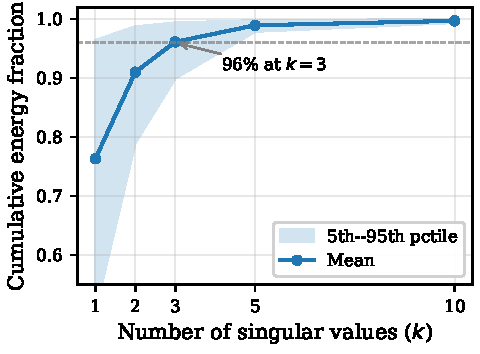
\includegraphics[width=\columnwidth]{../figures/fig1_sv_decay.pdf}
\caption{Cumulative energy fraction vs.\ number of singular values, averaged over 500~matchups (5th--95th percentile envelope). The top~3 singular values capture 96\% of spectral energy, revealing that VGC turn-1 is a 3-dimensional game in a ${\sim}122$-dimensional action space.}
\label{fig:sv}
\end{figure}

\textbf{Projection test.} We project BC--Nash deviation vectors onto $R$'s singular subspaces. For player~1, $\|U_k^\top \delta_p\|^2 / \|\delta_p\|^2$ measures the fraction of deviation energy in the top-$k$ column space (analogously for player~2). Only 7.1\% [6.8\%, 7.5\%] falls in the top-3 dimensions; 93\% of deviation energy lies in the payoff null space (Table~\ref{tab:projection}).

\begin{table}[t]
\caption{Deviation energy in top-$k$ SVD dimensions (500~matchups, 95\% bootstrap CI).}
\label{tab:projection}
\vskip 0.1in
\centering
\small
\begin{tabular}{lcc}
\toprule
$k$ & Energy in top-$k$ & In null space \\
\midrule
1 & 0.022 [0.021, 0.024] & 0.978 \\
3 & 0.071 [0.068, 0.075] & \textbf{0.929} \\
5 & 0.101 [0.098, 0.105] & 0.899 \\
10 & 0.151 [0.146, 0.156] & 0.849 \\
\bottomrule
\end{tabular}
\vskip -0.1in
\end{table}

\subsection{Interaction Decomposition}

Both players deviate massively from Nash, so why don't these deviations compound? The payoff gap between BC-vs-BC and Nash decomposes into three terms. Two are individual: player~1 benefits from player~2's suboptimality, and simultaneously pays a cost for their own. The third is a bilinear interaction between the two deviations. For convention to be free, we need these terms to cancel or be small. They are. Decomposing:
\begin{equation}
\underbrace{p_\text{BC}^\top R\, q_\text{BC}}_{\text{BC-vs-BC}} - V^* = \Delta_1 + \Delta_2 + \underbrace{(p_\text{BC} - p^*)^\top R\, (q_\text{BC} - q^*)}_{\text{interaction}}
\label{eq:decomp}
\end{equation}
where $\Delta_1 = {p^*}^\top R\, (q_\text{BC} - q^*)$ is the gain player~1 gets from player~2 deviating (positive, since Nash can exploit any deviation) and $\Delta_2 = (p_\text{BC} - p^*)^\top R\, q^*$ is the cost player~1 pays for their own deviation (negative, since Nash punishes deviation). The minimax theorem guarantees these signs, but their near-cancellation in magnitude is empirical: over 500 matchups, $\Delta_1 = +1.03$ and $\Delta_2 = -1.02$, with per-matchup std of 0.57. The interaction term is $-0.03$, small because the deviations $\delta_p, \delta_q$ are nearly orthogonal to $R$'s column and row spaces. In a full-rank game, two large deviations would produce a large cross-term. Here, because both deviations live almost entirely in the null space of $R$, their product through $R$ vanishes.

\textbf{Rank-reduction validation.} If the game is truly 3-dimensional, rank-$k$ approximations should preserve game-theoretic properties. Table~\ref{tab:rank_reduction} confirms this: rank-3 preserves 97.2\% of exploitability.

\begin{table}[t]
\caption{Game properties under rank-$k$ approximation (500~matchups).}
\label{tab:rank_reduction}
\vskip 0.1in
\centering
\small
\begin{tabular}{lccc}
\toprule
$k$ & Exploit ratio & $|\Delta V^*|$ & TV(Nash$_k$, Nash) \\
\midrule
1 & 0.756 & 0.444 & 0.850 \\
3 & \textbf{0.972} & 0.144 & 0.523 \\
5 & 0.993 & 0.053 & 0.374 \\
10 & 1.000 & 0.027 & 0.260 \\
\bottomrule
\end{tabular}
\vskip -0.1in
\end{table}

\textbf{Spectral bound.} Standard spectral arguments formalize why low rank implies small gaps. Let $R = R_k + E$ where $R_k$ is the best rank-$k$ approximation and $\|E\|_2 = \sigma_{k+1}$ by the Eckart--Young theorem \citep{eckart1936approximation}. For any strategy pair $(p, q)$: $|p^\top R\, q - V^*| \leq |p^\top R_k\, q - V^*_k| + 2\sigma_{k+1}$, where $V^*_k$ is the Nash value of $R_k$. Both the perturbation term and the Nash-value shift are bounded by $\sigma_{k+1}$ via $|p^\top E\, q| \leq \|E\|_2 \leq \sigma_{k+1}$ for probability vectors. For VGC with $k = 3$ and $\sigma_4 / \sigma_1 \approx 0.04$, the empirical gap of 0.02 sits well within this bound.

\textbf{Robustness to model capacity.} Low rank could be an artifact of the dynamics model's bottleneck. We test across three action-embedding capacities ($d = 32, 64, 128$). Effective rank increases only from 2.9 to 4.3, and the highest-capacity model has worse validation loss (526 vs.\ 445), suggesting extra dimensions reflect overfitting. The two well-fit models agree on effective rank within $\pm 1$ for 93\% of matchups. Payoff-weighted TV is stable at 0.019 across all capacities. Low rank is a property of VGC, not the model.

%% ============================================================
\section{Where Convention Fails: Terastallization}
\label{sec:tera}
%% ============================================================

There is one dimension where convention is costly. Terastallization is an irreversible resource in VGC: once used, it is gone for the rest of the game, and a typical VGC match lasts 8--15 turns. From a multi-turn perspective, conserving tera is rational. Later turns may present better opportunities---a weakened opponent that tera could finish off, or a defensive type change that could survive a critical hit. Waiting also gives you more information about your opponent's plan, letting you tera reactively rather than speculatively. Experts follow this logic, and it is reflected in the data: BC uses tera on turn~1 in only 25\% of matchups. But our turn-1-only model, which evaluates each turn in isolation with no access to future states, says the opposite. Optimal play uses tera 99\% of the time, because in a single-turn game there is no ``later'' to save it for.

\textbf{Magnitude.} Restricting the best response to BC's tera class (same tera/no-tera choice) reduces exploitability by 0.41 reward units, or 30\% of total exploitability [29\%, 32\%]. No other single decision contributes as much.

\textbf{Aggression.} Beyond tera, best responses target opponents 79\% of the time vs.\ 52\% for BC. The joint action pattern shifts from balanced (27\% both-offensive, 50\% mixed, 23\% both-support under BC) to heavily offensive (65\% both-offensive, 29\% mixed, 6\% both-support under BR). Figure~\ref{fig:tera} visualizes both contrasts.

\begin{figure}[t]
\centering
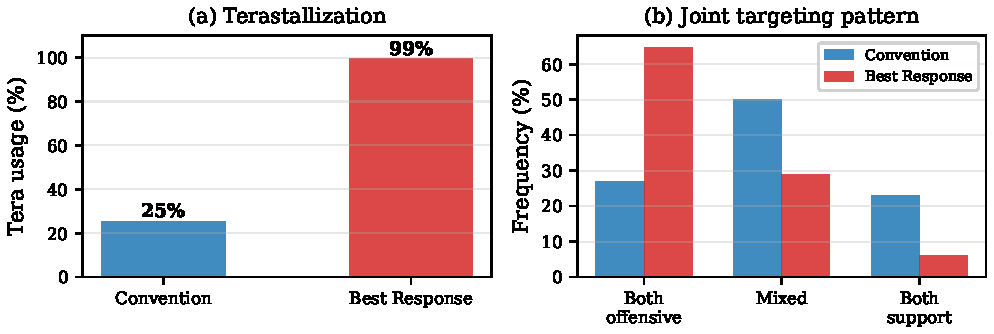
\includegraphics[width=\columnwidth]{../figures/fig2_tera_aggression.pdf}
\caption{Behavioral differences between conventional (BC) and optimal (BR) play. \textbf{(a)}~Best responses terastallize almost universally (99\%) while experts conserve tera for later turns (25\%). This single binary decision accounts for 30\% of total exploitability. \textbf{(b)}~Optimal play is systematically more aggressive, shifting the joint action pattern from balanced to heavily offensive. Tera conservation and passive targeting account for most of the gap between convention and myopic optimality.}
\label{fig:tera}
\end{figure}

\textbf{Case study.} Consider a Calyrex-Ice / Ogerpon-Hearthflame lead facing Kyurem-White / Maushold. BC plays Trick Room + Follow Me with 49\% probability, a purely defensive setup targeting self, for a payoff of $-0.75$. Nash concentrates 87\% on High Horsepower + Horn Leech, both targeting the opponent's Maushold slot, with tera, for a payoff of $+2.75$. The best response copies this aggressive targeting (payoff $+2.76$ against BC), a swing of 3.51, the largest in our sample. Convention learned a defensive posture (Trick Room to reverse speed, Follow Me to redirect attacks) when the game demands immediate aggression. BC never terastallizes in its top action; Nash always does. BC targets self in every top action; Nash targets the opponent exclusively.

\textbf{Domain interpretation.} Experts rationally conserve tera for later turns when they might have more information; our turn-1-only game theory says use it now. A player who terastallizes early reveals their type change to the opponent and cannot adapt defensively to late-game threats --- if a sweeper survives to the endgame, a well-timed defensive tera could be the difference between winning and losing. Saving tera also means waiting for more information: later turns reveal the opponent's plan, letting you tera reactively rather than on a guess. This gap between myopic and far-sighted optimality explains the 30\% contribution and suggests it would shrink in a multi-turn analysis. A regression of exploitability on structural features yields $R^2 = 0.08$. The \emph{direction} of exploitation is systematic (tera + aggression), but the \emph{magnitude} is matchup-specific.

\textbf{Empirical validation.} Battle-outcome data from 124,087 full battles quantifies the cost of early tera. Players who terastallize on turn~1 win 51.2\% [50.9, 51.6] of the time; those who defer tera to a later turn win 48.9\% [48.7, 49.2]. In head-to-head matchups where one player teras turn~1 and the other defers, the early user wins 51.7\% ($n = 45{,}172$). The advantage is statistically significant, comparable to side selection in MOBAs (${\sim}2$pp), but modest: our horizon-1 model prescribes tera 99\% of the time because it sees large immediate payoff gains, yet those gains translate to fewer than two extra wins per hundred battles. The tactical value of early tera is real but largely offset by the option value of waiting. Early tera is not punished; conservation is not costly either, since experts who defer can deploy tera reactively when it matters most.

%% ============================================================
\section{Can Reward Optimization Escape Convention?}
\label{sec:cql}
%% ============================================================

Every result so far uses imitation learning. Perhaps convention persists only because BC never has reason to escape it. We test this with Conservative Q-Learning (CQL) \citep{kumar2020conservative} on the same dataset. CQL penalizes Q-values on out-of-distribution actions, which matters here because the action space is ${\sim}200$ and most actions are never observed in any given matchup. Without the penalty, a na\"ive Q-learner would overestimate unseen actions and produce a degenerate policy. Because our horizon is one step, CQL reduces to conservative reward regression with no bootstrapping or target networks. We use a factored Q-function $Q(s,a) = Q_a(s,\text{slot}_a) + Q_b(s,\text{slot}_b) + Q_\text{tera}(s,\text{tera})$ with the same encoder architecture as BC. The factored decomposition is justified by the near-zero mutual information between leads (0.018~bits). CQL can improve on expert behavior where the reward signal supports it, but stays anchored to the data distribution.

\begin{table}[t]
\caption{BC vs.\ CQL vs.\ Nash (500 matchups, 95\% CI).}
\label{tab:cql}
\vskip 0.1in
\centering
\small
\begin{tabular}{lccc}
\toprule
Metric & BC & CQL & Nash \\
\midrule
Exploitability & 1.40 [1.36, 1.46] & 1.15 [1.08, 1.23] & 0.00 \\
TV($\cdot$, Nash) & 0.99 & 0.98 & 0.00 \\
Worst-case value & $-1.23$ & $-0.99$ & $+0.16$ \\
\bottomrule
\end{tabular}
\vskip -0.1in
\end{table}

CQL reliably reduces exploitability (411 of 500 matchups, $p < 10^{-51}$), narrowing the gap by 17\% overall (1.40 $\to$ 1.15) and improving worst-case value by 20\%. But both policies remain TV $= 0.98$ from Nash. The improvement is uneven: CQL reduces exploitability by 26\% in the most-exploitable quartile and near 0\% in the least. This gradient matches the low-rank theory; matchups with higher exploitability have more payoff-relevant variation for the reward signal to exploit.

Projecting the CQL--BC difference onto the SVD basis confirms this: 94\% of the distributional shift lies in the payoff null space, with only 6\% in the top-3 payoff-relevant dimensions. Behaviorally, CQL's largest shift is in terastallization. It doubles the tera rate from 28\% to 54\% (Nash: 95\%) and increases offensive targeting from 50\% to 65\% (Nash: 69\%). This is consistent with \S\ref{sec:tera}: tera is the one dimension where convention is costly, so reward optimization correctly shifts probability mass there. But even this shift captures only half the Nash tera rate --- the conservative penalty keeps CQL tethered to the data distribution.

The two policies are meaningfully different (TV(CQL, BC) $= 0.60$), yet 94\% of that movement is payoff-irrelevant. CQL finds a \emph{different convention}, not a better strategy --- it rearranges probability mass extensively, but almost entirely within the null space where rearrangement has no payoff consequence. Convention persists because the game's low-rank structure leaves little room for \emph{any} objective to find improvement, not because imitation is the wrong objective.

%% ============================================================
\section{Ablations and Additional Measurements}
\label{sec:ablations}
%% ============================================================

\textbf{Autoregressive BC.} An autoregressive variant with $P(a_2 \mid a_1)$ yields identical exploitability (1.41 $\to$ 1.41). Mutual information between leads' actions is 0.018~bits (effectively independent), validating the factored assumption.

\textbf{Improved dynamics.} The dyn\_002 model ($d_\text{action} = 64$, lower validation loss) finds \emph{more} exploitability (1.41 $\to$ 1.52). Our base estimate is a lower bound.

\textbf{QRE rejection.} Quantal response equilibrium \citep{mckelvey1995quantal} fits poorly. 92\% of matchups have best-fit $\lambda \leq 0.01$ (essentially uniform), and TV(QRE, BC) $= 0.68$. Experts are far more structured than ``noisy Nash.''

\textbf{Reward sensitivity.} Our payoff weights ($w_\text{hp} = 1$, $w_\text{ko} = 3$, $w_\text{field} = 0.5$) are domain-informed heuristics. We recompute all game-theoretic quantities under $w_\text{ko} \in \{1, 3, 5\}$ with other weights fixed (Table~\ref{tab:reward_sens}). Exploitability scales with the weight, but the cross-play gap remains indistinguishable from zero at all settings, so our main result is not an artifact of the reward specification.

\begin{table}[t]
\caption{Reward sensitivity: game-theoretic quantities under varying KO weight (500~matchups, 95\% CI).}
\label{tab:reward_sens}
\vskip 0.1in
\centering
\small
\begin{tabular}{lccc}
\toprule
$w_\text{ko}$ & Exploitability & BC-vs-BC $- V^*$ & Convention free? \\
\midrule
1.0 & 0.58 [0.56, 0.60] & $+0.02$ [$-0.01$, $0.04$] & Yes \\
3.0 & 1.41 [1.36, 1.46] & $-0.02$ [$-0.07$, $0.04$] & Yes \\
5.0 & 2.25 [2.16, 2.33] & $-0.05$ [$-0.13$, $0.04$] & Yes \\
\bottomrule
\end{tabular}
\vskip -0.1in
\end{table}

\textbf{Payoff-weighted TV.} Reweighting TV distance by each action's contribution to payoff variance collapses the distance from 0.99 to 0.019, a 50$\times$ reduction confirming that BC--Nash divergence is concentrated in payoff-irrelevant dimensions.

\textbf{Smoothed best-response dynamics.} Smoothed best response iteratively updates each player's strategy toward a best response to the opponent's current mix, with a step size that prevents oscillation. Initialized at BC, it converges from exploitability 2.81 to below 0.50 in 19 iterations, reaching 0.14 by iteration~500 (Figure~\ref{fig:br}). With only ${\sim}3$ effective dimensions, the dynamics converge quickly --- most of the strategy space is irrelevant to the optimization.

\textbf{Mixture interpolation.} Blending BC toward Nash via $p_\alpha = (1{-}\alpha)\,p_\text{BC} + \alpha\,p^*$ yields a nearly perfect linear decay in exploitability. $\text{exploit}(\alpha) \approx 1.41 - 1.41\alpha$ ($R^2 = 0.9995$). There is no phase transition, no threshold $\alpha$ at which exploitability suddenly drops, consistent with 93\% of the BC--Nash gap lying in the payoff null space. In a high-rank game, one would expect diminishing returns (early corrections fix the most exploitable dimensions first) or sharp transitions (a critical mass of corrections suddenly closes off exploitation). The linearity is a consequence of low rank: with so few payoff-relevant directions, every step toward Nash buys the same marginal improvement. There is nothing to ``unlock.''

\begin{figure}[t]
\centering
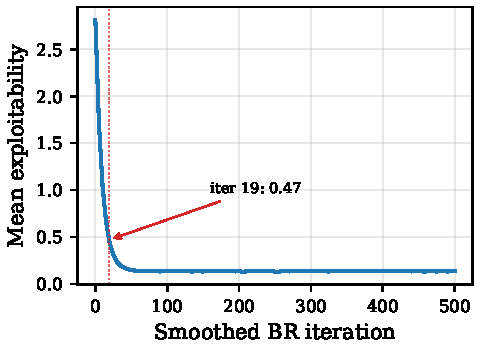
\includegraphics[width=\columnwidth]{../figures/fig3_smoothed_br.pdf}
\caption{Smoothed best-response convergence from BC initialization. Exploitability decreases from 2.81 to below 0.50 in ${\sim}19$ iterations, reaching 0.14 at iteration~500. Convergence is fast because only ${\sim}3$ payoff-relevant dimensions need correcting.}
\label{fig:br}
\end{figure}

%% ============================================================
\section{Discussion}
\label{sec:discussion}
%% ============================================================

Convention costs 1.41 reward units against an optimizer but 0.00 against another conventional player. The game's low-rank structure (effective rank~3 out of ${\sim}122$ actions) means 93\% of strategic variation lies in the payoff null space. You can be wrong in 119 out of 122 dimensions and it does not matter. Switching from imitation to reward optimization (CQL) narrows exploitability by 17\% without closing the gap. The game is forgiving, and expert skill has little to do with it.

\textbf{Convention at every stage.} Our companion project TurnZero \citep{brennan2026turnzero} found that expert team selection during the pre-battle preview also reflects convention rather than strategic optimization (opponent contributes $-1.3$pp to prediction accuracy). Turn-1 actions follow the same pattern. The game's low-rank structure, which we attribute to the dominance of a few factors (type advantage, raw power, speed tier) over hundreds of nominal action combinations, makes convention free at both stages.

\textbf{The tera exception.} Terastallization accounts for 30\% of exploitability despite being a single binary decision. Unlike move selection, which lives in the payoff null space, tera is irreversible with multi-turn consequences. The tension between myopic and far-sighted optimality is the main limitation of our turn-1 framework.

\textbf{Beyond Pok\'emon.} Action redundancy makes convention free; irreversibility makes it costly. This pair of conditions yields a testable prediction. In games where the payoff matrix has low effective rank relative to its nominal size, conventional play should be near-optimal even when it looks nothing like Nash. Real-time strategy games, where many unit compositions achieve similar outcomes, and sports play-calling, where most play variations are functionally equivalent against a given defense, are natural candidates. Conversely, convention should be costly wherever irreversible resource commitments dominate: poker all-ins that risk elimination, military reserve deployments, or auction bids that lock in capital. Irreversible decisions cannot hide in the null space because they change the game state permanently. Existing explanations for suboptimal play, such as QRE and level-$k$, locate the problem in the player's rationality. Spectral decomposition locates it in the game itself: if the payoff matrix has low rank, most deviations are irrelevant regardless of why players deviate. The question is not whether humans are rational, but whether the game notices.

\textbf{Limitations.} (a)~Turn-1 only: multi-turn consequences, especially for tera, are not captured. Turn-1 reward predicts only 4\% of win variance ($r = 0.21$); our analysis covers a narrow but structurally informative slice of the game. A lost Pok\'emon also grants a free switch-in, so a turn-1 KO that our reward model scores negatively may actually set up a sweep. (b)~Dynamics model noise (SNR 3.4:1) is the primary methodological constraint. (c)~The cross-play gap averages to zero but shows heterogeneity (std 0.65 per matchup); this cancellation is empirical, not a mathematical identity. (d)~Regulation~G specific; the low-rank hypothesis is testable in other formats. (e)~Later turns with switching present higher effective rank, an open question.

\bibliography{references}
\bibliographystyle{icml2018}

\end{document}
